\section{Experiments}
I performed experiments to evaluate the performances of similarity measures and algorithms in Section~\ref{sec:connectionsimilarity}.
\newline
In Section~\ref{subsec:datasetandsetup}, I describe the dataset that I used for the experiments.\newline
In Section~\ref{subsec:preprocessing}, I describe data pre-processing over the dataset.\newline
In Section~\ref{subsec:detectinganomalies}, I evaluate how successful the algorithms are in detecting different types of anomalies.

\subsection{Dataset and Setup}
\label{subsec:datasetandsetup}
The KDD 99 dataset is mainly used for a network-based intrusion detection algorithm evaluation. 
I select the NSL-KDD dataset \cite{tavallaee09}, an up-to-date version of the KDD 99 dataset, as an effective benchmark. 
% Since the NSL-KDD dataset solves issues in the KDD 99 dataset, I use the dataset as an effective benchmark. 
Its relevance of each feature in the dataset is also studied \cite{olusola10} \cite{kayacik05}. 
% All source code is on the Internet. 
% I use NSL-KDD99 Dataset for the report. 
% semi-supervised approach

\begin{figure}[htb2]
\begin{center}
%\begin{inparaenum}[\itshape a\upshape)]
%\item data preprocessing
%\item data transformation
%\item affinity matrix computation
%\item clustering
%\item outlier detection
%\end{inparaenum}
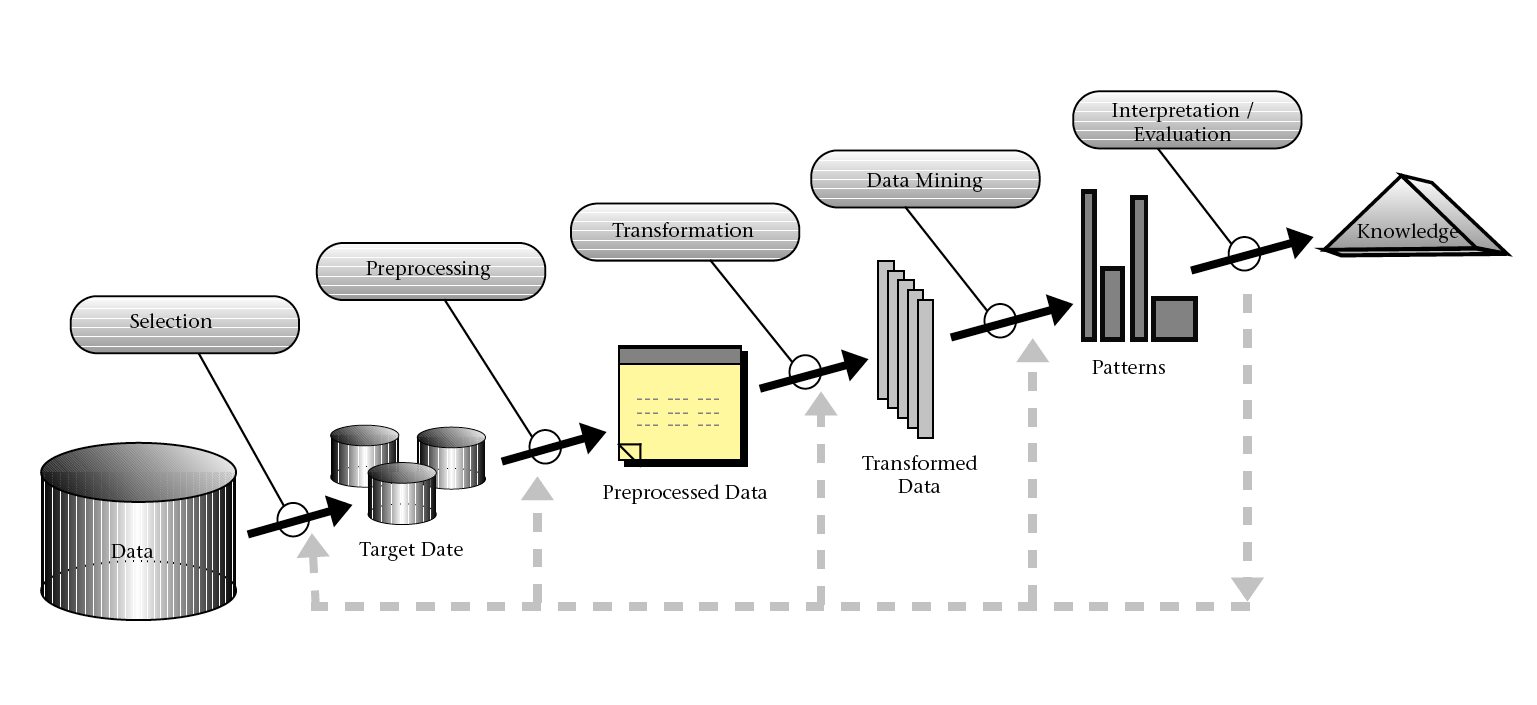
\includegraphics[width=5.5in,angle=0]{./sections/Fayyad96kdd-process.eps}
\end{center}
\caption{Overview of Knowledge Discovery System}
\label{fig:refSingleRobot1}
\end{figure}
The intrusion detection system should find specific kinds of abnormal traffic e.g. a denial of service (DoS) attack. 
Moreover it should check if these new sets of monitoring network traffic show similar properties as the original data or not. 
I construct the system similar to the knowledge discovery system \cite{fayyad96} because it is widely used among intrusion detection systems. 
A proposed approach to construct a pairwise similarity matrix is that it utilizes cosine similarity between score vectors of two data points as in Section~\ref{subsec:normalabnormalsimilarity}. 
In order to achieve this, the system includes GMM of attributes, protocols and classes. %to construct a vector consists of log-likelihood scores for a data point. 
%The EM approach is used to fit those models and is guaranteed to converge to a local optimum on given input. 
%With those components, we can make a score vector for a data point and those scores are weighted based on their importance in the dataset \cite{kayacik05}.
%to get 2D data where x-axis is a score for normal connection similarity and y-axis is a score for known abnormal connection similarity. 
The experiment suggests that such local optimum can effectively separate different connections and most of unknown classes. 
%\begin{figure}[htb2]
%\begin{center}
%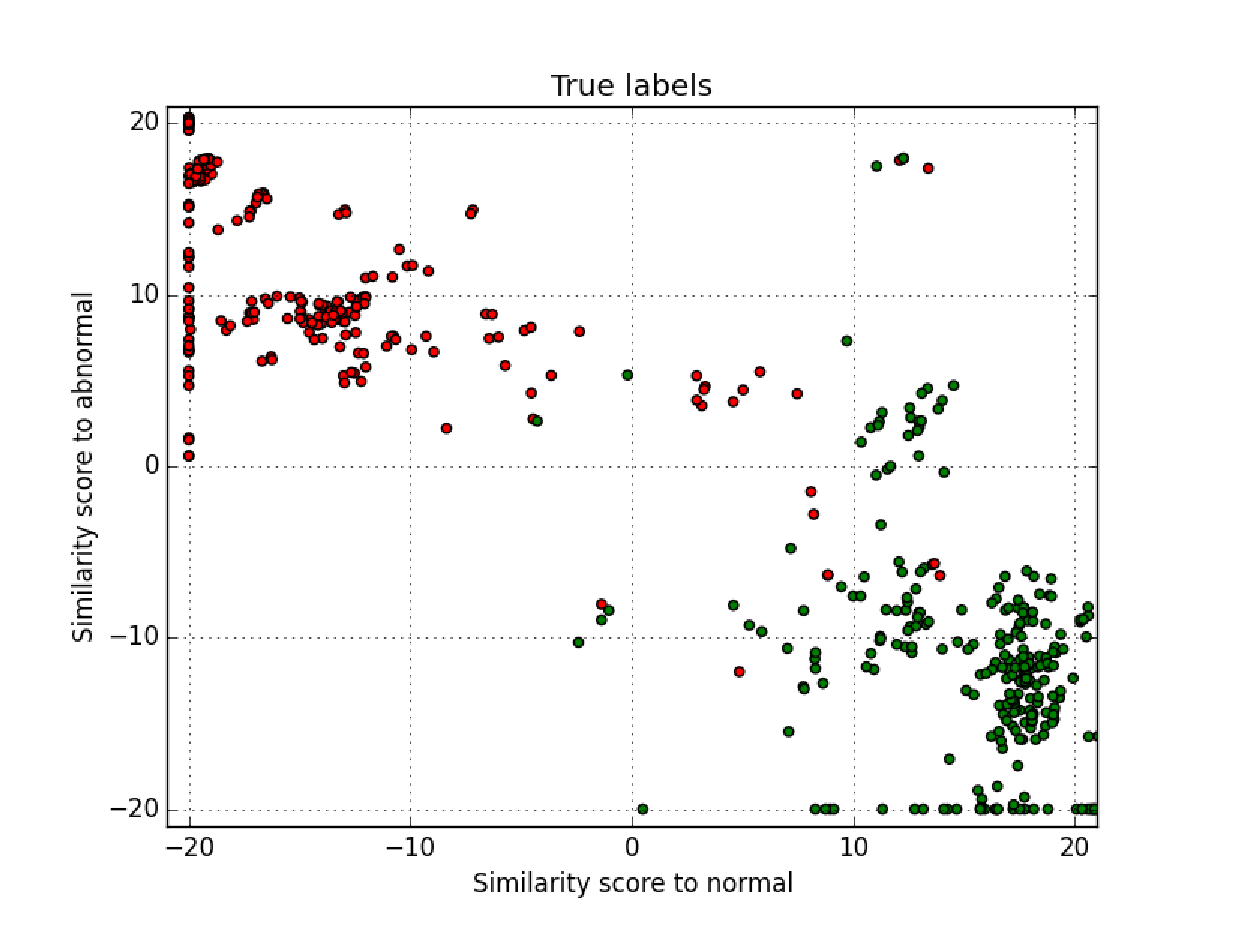
\includegraphics[width=3.5in,angle=0]{./sections/training20_only_true_.eps}
%\end{center}
%\caption{Similarity of normal and abnormal connections in training set.}
%% The left figure shows data points including known anomalies and the right known type of anomalies shows data points including unknown type of anomalies.} % I may show rest of data in appendix
%\label{fig:refSingleRobot1}
%\end{figure}

%In order for spectral anaysis, we need to make a sparse affinity matrix from transported data. 
%We can compute a sparse affinity matrix from a pairwise similarity matrix. 
After we have a pairwise similarity matrix, one way to convert similarity matrix to a sparse affinity matrix is that dealing with the affinities for $k$ nearest neighborhood, and set all other values for current data point to zero. 
I choose $k = 8$ because it is commonly used in spectral clustering approaches. 

% Altho require non-convex boundaries,
%\subsection{Computing affinity matrix}
%%The processing steps of the approach can be summerized as follows:
%%1) Training mixture model with training set containing records of both normal and anomalous connections.
%%2) The data are divided into different clusters for normal and anomalous connections using Spectral clustering algorithm.
%\subsubsection{Data pre-processing}
%\begin{itemize}
%\item categorical value to integer e.g.) service-type (ftp-data,http,etc).
%\item log of big number e.g.) duration, src-bytes.
%\end{itemize}
%\subsubsection{Affinity matrix computation}
%The data points are associated with each other by pairwise similarity.
%\begin{itemize}
%\item Construct similarity matrix with distance metric.
%\item Construct affinity matrix from similarity matrix with 8-nearest neighbors algorithm.
%\end{itemize}
%\subsection{Clustering}
%%\subsubsection{Number of clusters prediction}
%%Predict number of clusters based on the eigengap.
%%\subsubsection{Spectral clustering algorithm}
%%Normalized cut algorithm. \cite{jianbo00}
%%\subsubsection{Representative of clusters}
%%Clusters are represented by the mean and variance.
%\subsection{Detecting anomaly from clusters}
%%Distance based outlier detection is used.
%%\begin{itemize}
%%\item It do not require any prior knowledge.
%%\item k-nearest neighbor outlier detection algorithm. \cite{knorr00}
%%\end{itemize}

\subsection{Data Pre-processing}
\label{subsec:preprocessing}
A set of network connections $D_{\text{train}=(d_1, \cdots, d_{25192})}$ and $D_{\text{test}=(d_1, \cdots, d_{11850})}$ can be extracted from the NSL-KDD dataset. 
Each connection $x_i = (y, (\lambda_{1}, \cdots, \lambda_{39}))$ consists of a class label \\ 
$y \in Y=\{\text{normal},\text{anomaly}_1,\cdots,\text{anomaly}_{34}\}$ and an attribute vector $(\lambda_1,\cdots,\lambda_{39})$. 

$D_{\text{train}}$ has 22 types of known anomaly and $D_{\text{test}}$ has 39 types of known and unknown anomaly which can be seen in Table~\ref{fig:anomalyclasses}. 
Three of feature attributes are categorical values and ten of them are large numbers which requires data pre-processing. 
Preprocessing work does convert three of them from categorical values into integer values and apply $\ln$ function on large numbers. 
Each attributes' probability density can be estimated by EM algorithm that can be used to calculate a log-likelihood as in Section~\ref{subsec:normalabnormalsimilarity}. 

%Those of three are converted from categorical values into integer values. 
%Preprocessing work applies log probability on large numbers $\hat{\lambda_{j}} = \log (\lambda_{j})$ where $j$ is an index of large number attributes. 
\begin{table}[h]
\begin{center}
\begin{tabular}{| l | p{10cm} |}
\hline
Type of Attributes & Attributes Names \\
\hline
Categorical values (3) & attack, service, flag \\
\hline
Large numbers (10) & duration, src-bytes, dst-bytes, num-root, num-compromised, num-file-creations, count, srv-count, dst-host-count, dst-host-srv-count \\
\hline
Others (26) & land, wrong-fragment, urgent, hot, num-failed-logins, logged-in,su-compromised, root-sheel, su-attempted, num-shells, num-access-files, num-outbound-cmds, is-host-login, is-guest-login, serror-rate, srv-serror-rate, rerror-rate, same-srv-rate, diff-srv-rate, srv-diff-host-rate, dst-host-same-srv-rate, dst-host-diff-srv-rate, dst-host-serror-rate, dst-host-srv-serror-rate, dst-host-rerror-rate, dst-host-srv-rerror-rate \\
\hline
\end{tabular}
\end{center}
\caption{39 attributes in the NSL-KDD dataset.} % Preprocessing work required on categorical values or large numbers.
\label{fig:preprocessing}
\end{table}

Given those mixture models, we can get 2-dimensional vector $\hat{x} = (s_{\text{normal}}, s_{\text{abnormal}})$ 
where $s_{\text{normal}}$ is a score generated from 39 mixture models of normal network connections of protocol $p$ 
and $s_{\text{abnormal}}$ is a score generated from 39 mixture models of abnormal network connections of protocol $p$. 
Each data point $x$ is assigned to protocol $p \in \{\text{TCP/IP}, \text{ICMP}, \text{UDP}\}$ 

With those transported points $\hat{x}$, we can construct an affinity matrix with cosine similarity function as in Section~\ref{sec:spectralclustering}. 
Therefore it is ready to use spectral clustering. 

\subsection{Detecting Anomalies}
\label{subsec:detectinganomalies}
In this section, I describe how a sparse affinity matrix can be used to detect point and collective anomalies. 
I divide the testset into known anomalies and unknown anomalies in the following experiments. 
To use spectral clustering, we need enough sample data apart from anomalies to construct an affinity matrix. 
I use 2000 random samples of the NSL-KDD dataset. 
Usually half of them are normal while the others are abnormal. 
Here is a sample data that I use in this experiments and a result of algorithm given sample data. 

\begin{table}[h]
\begin{center}
\scalebox{0.7}{
\begin{tabular}{| l | l | l | l | l | l | p{5cm} |}
\hline
Total number of samples & The number of anomalies & TP & TN & FP & FN & Detection rate $\%$ correct \\
\hline
2000 & 962 & 1021 & 907 & 55 & 17 & 94.2 \\ 
\hline
\end{tabular}
}
\end{center}
\caption{Detection result of sample data}
\label{fig:refSingleRobot1}
\end{table}

\subsubsection{Known Anomalies}
We can see that trained normal and abnormal similarity functions are sensitive to known anomalies in the testset.
%Their scores are similar to known anomalies and dissimilar to known normal network connections. 
For most of normal and abnormal classes, similarity scores of their data points are very close to known normal or abnormal connections. 
%normal and abnormal connections similarity are sensitive to known anomalies. 
It shows how much trained similarity functions capture the effects of known anomalies. 
% The similarity coputed by mixture models gives similarity scores that are used to find k nearest neighborhood.
%In summary, all the class successfully detect known anomalies in spectral approach. 
However this approach does not work if the number of intrusions are insufficient because those classes are not well trained in mixture models, and data points tend to assigned to different clusters. 
For example, detection rates are poor to the classes that has less than 100 data points such as \textit{ftp write} and \textit{rootkit} in Table~\ref{fig:knownanomaliesdetectionrate}. 

\begin{figure}[htb2]
\begin{center}
\subfloat[Predicted labels]{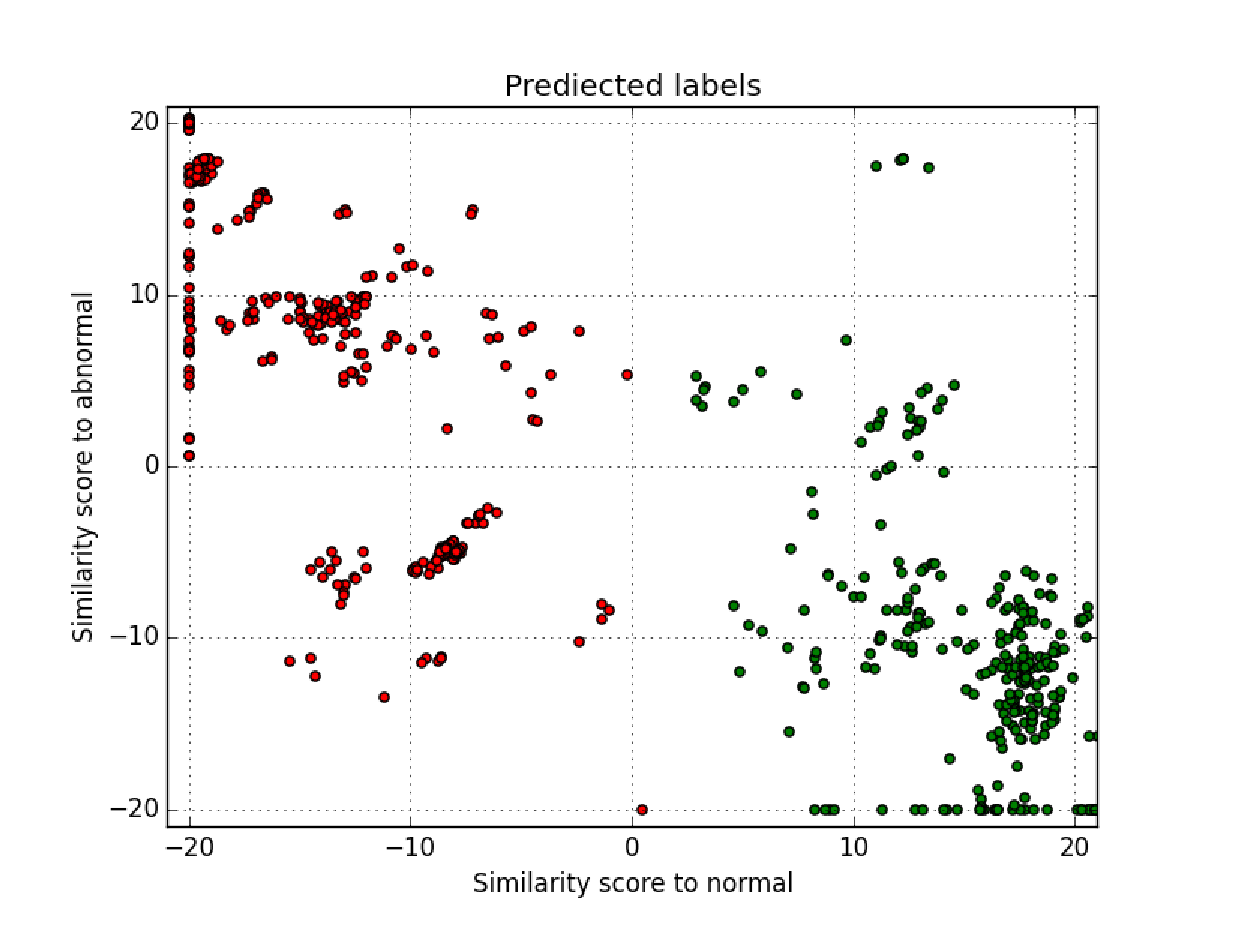
\includegraphics[width=3.0in,angle=0]{./sections/training20_test20_back_prediction_.eps}}
\subfloat[True labels]{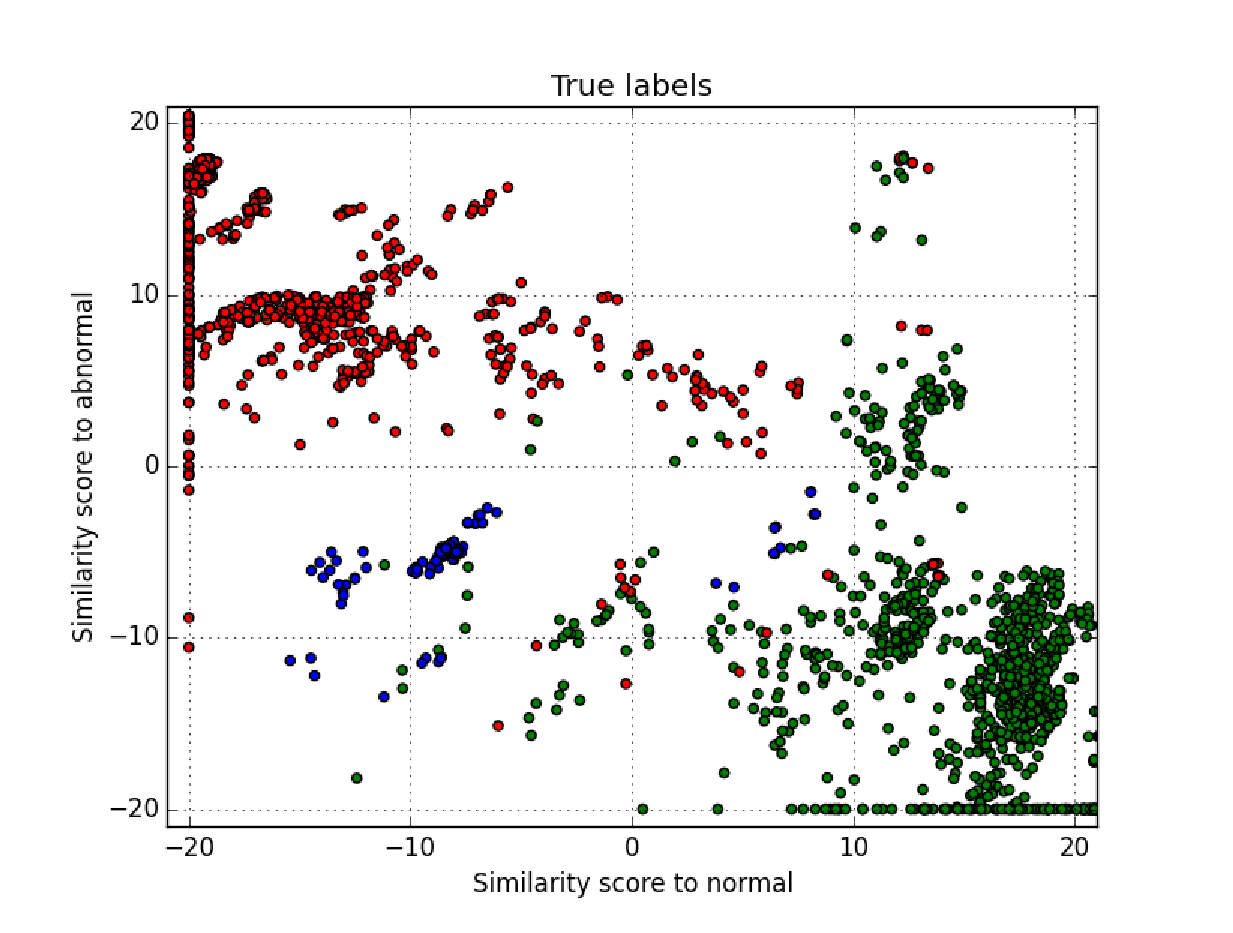
\includegraphics[width=3.0in,angle=0]{./sections/training20_test20_back_true_.eps}}
\end{center}
\caption{Anomaly detection for known anomalies. Red:Known and seen abnormal connections, Green:Known and seen normal connections, Blue:Intrusion \textit{back} which is a known and unseen anomalies.} % I may show rest of data in appendix
\label{fig:refSingleRobot1}

\end{figure}
\begin{table}[!ht]
\begin{center}
\begin{singlespace}
\scalebox{0.7}{
\begin{tabular}{| l | l | l | l | l | l | p{5cm} |}
\hline
Type of Anomaly & The number of anomalies & TP & TN & FP & FN & Detection rate $\%$ correct \\
\hline
guess passwd & 2193 (1231) & 898 & 2158 (1231) & 35 (0) & 140 & 98.4 (100) \\
\hline
ftp write & 965 (3) & 1019 & 921 (1) & 44 (2) & 19 & 95.44 (33.3) \\
\hline
nmap & 1038 (73) & 1002 & 997 (73) & 38 (0) & 36 & 96.53 (100) \\
\hline
back & 1332 (370) & 1011 & 1280 (358) & 41 (12) & 27 & 96.8 (96.7) \\
\hline
multihop & 980 (18) & 1011 & 937 (15) & 43 (3) & 27 & 95.6 (83.3) \\
\hline
rootkit & 975 (13) & 1019 & 920 (0) & 55 (13) & 19 & 94.3 (0)  \\
\hline
pod & 1003 (41) & 1013 & 963 (41) & 40 (0) & 25 & 96 (100) \\
\hline
perl & 964 (2) & 1021 & 907 (0) & 57 (2) & 17 & 94 (0) \\
\hline
ipsweep & 1169 (207) & 999 & 1041 (184) & 62 (23) & 39 & 94.37 (88.8) \\
\hline
teardrop & 974 (12) & 1021 & 932 (12) & 42 (0) & 17 & 95.68 (100) \\
\hline
satan & 1741 (779) & 1015 & 1657 (777) & 40 (2) & 23 & 97.6 (99.7) \\
\hline
loadmodule & 964 (2) & 1011 & 924 (2) & 40 (0) & 27 & 95.8 (100)  \\
\hline
buffer overflow & 982 (20) & 1012 & 940 (16) & 42 (4) & 26 & 95.7 (80) \\ 
\hline
phf & 964 (2) & 1019 & 908 (1) & 56 (1) & 19 & 94.1 (50)  \\
\hline
warezmaster & 1906 (944) & 946 & 1834 (908) & 72 (36) & 92 & 96.2 (96.1) \\ 
\hline
imap & 963 (1) & 1019 & 907 (0) & 56 (1) & 19 & 94.1 (0) \\
\hline
warezclient & 984 (22) & 1019 & 907 (0) & 55 (22) & 19 & 94.2 (0) \\
\hline
land & 969 (7) & 1021 & 914 (7) & 55 (0) & 17 & 94.32 (100)  \\
\hline
neptune & 6293 (5331) & 933 & 5588 (5327) & 31 (4) & 105 & 99.4 (99.9) \\
\hline
smurf & 1627 (665) & 1018 & 1579 (665) & 48 (0) & 20 & 97 (100)  \\
\hline
\end{tabular}
}
\end{singlespace}
\end{center}
\caption{Detection result of known anomalies. The number in parentheses refers specific anomaly type.}
\label{fig:knownanomaliesdetectionrate}
\end{table}

%Result provides the sensitivity and the coverage of similarity measure that is effective. 
%All data point in testset for 21 known abnomal classes shows similar to known anomalies. 
%After it calcurate the similarity among data points 
%\begin{table}[h]
%\begin{center}
%\begin{tabular}{| l | l | l | p{5cm} |}
%\hline
%Type of Anomaly & Predicted normal & Predicted anormalies & $\%$ correct\\
%\hline
%True normal &  &  & \\
%\hline
%True anormalies &  &  & \\
%\hline
%\end{tabular}
%\end{center}
%\caption{Abnomal classes in NSL-KDD99}
%\label{fig:refSingleRobot1}
%\end{table}
% The detection rate for them are quite high. 
%
%\begin{figure}[htb2]
%\begin{center}
%\end{center}
%\caption{Clusters of connections including known anomalies. The x-axis shows the normal similarity scores and the y-axis shows the known abnormal similarity scores}
%\label{fig:refSingleRobot1}
%\end{figure}
\newpage
\subsubsection{Unknown Anomalies}
We see that normal and abnormal connection similarity are also sensitive to 13 of out 17 unknown anomalies. 
Although we also have four classes that are similar to normal connections, 
density measurement can detect those anomalies if it is above its threshold. 

13 unknown anomalies such as \textit{processtable} class are similar to known anomalies. 
Therefore we can detect them with exactly same way what it has done to known anomalies. 
Those results are good as known anomalies. 

\begin{table}[h]
\begin{center}
\scalebox{0.7}{
\begin{tabular}{| l | l | l | l | l | l | p{5cm} |}
\hline
Type of Anomaly & The number of anomalies & TP & TN & FP & FN & Detection rate $\%$ correct \\
\hline
processtable & 1647 (685) & 1018 & 1597 (683) & 50 (2) & 20 & 96.9 (99.7) \\ 
\hline
named & 979 (17) & 1021 & 924 (4) & 55 (13) & 17 & 94.3 (23.5) \\
\hline
udpstorm & 964 (2) & 1011 & 924 (2) & 40 (0) & 27 & 95.8 (100) \\
\hline
sqlattack & 964 (2) & 1021 & 907 (0) & 57 (2) & 17 & 94.0 (0)  \\
\hline
ps & 977 (15) & 1019 & 910 (3) & 67 (12) & 19 & 93.1 (20) \\
\hline
httptunnel & 1095 (133) & 1015 & 1016 (109) & 79 (24) & 23 & 92.7 (81.9)  \\
\hline
apache2 & 1699 (737) & 1014 & 1656 (734) & 43 (3) & 24 & 97.4 (99.5) \\
\hline
saint & 1281 (319) & 1014 & 1227 (309) & 54 (10) & 24 & 95.7 (96.8) \\
\hline
mscan & 1958 (996) & 1018 & 1910 (996) & 48 (0) & 20 & 97.5 (100) \\
\hline
xterm & 975 (13) & 1011 & 935 (13) & 40 (0) & 27 & 95.8 (100)  \\
\hline
worm & 964 (2) & 1019 & 907 (0) & 57 (2) & 19 & 94.0 (0) \\
\hline
xlock & 971 (9) & 1013 & 925 (3) & 46 (6) & 25 & 95.2 (66.66)  \\
\hline
xsnoop & 966 (4) & 1013 & 925 (3) & 41 (1) & 25 & 95.7 (75)  \\
\hline
\end{tabular}
}
\end{center}
\caption{Detection result of unknown anomalies that is similar to the known anomalies detection rate. The number in parentheses refers specific anomaly type.}
\label{fig:refSingleRobot1}
\end{table}

We have four classes that are close to the normal connections. 
In that case, a cluster resulted by spectral clustering is denser than normal case, so it can be detected by density based algorithm if we compare with mixture density generated by normal connections only. 
So with those prior knowledge we can use a spectral approach to find abnormal clusters which is originally classified as normal clusters. 

\begin{figure}[htb2]
\begin{center}
\subfloat[Predicted labels]{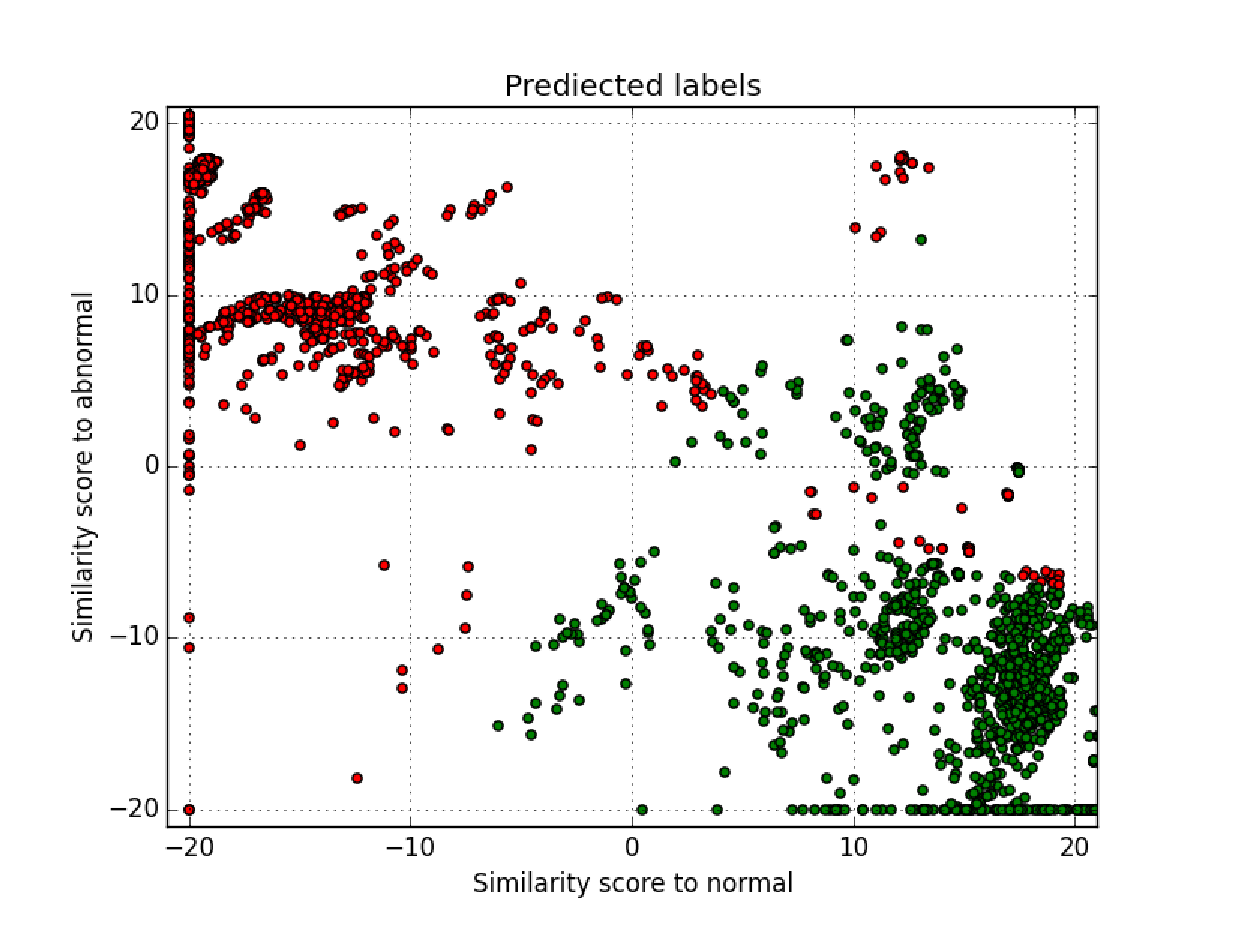
\includegraphics[width=2.0in,angle=0]{./sections/training20_test20_snmpguess_prediction_.eps}}
\subfloat[True labels]{\includegraphics[width=2.0in,angle=0]{./sections/training20_test20_snmpguess_true_.eps}}
\subfloat[Densities]{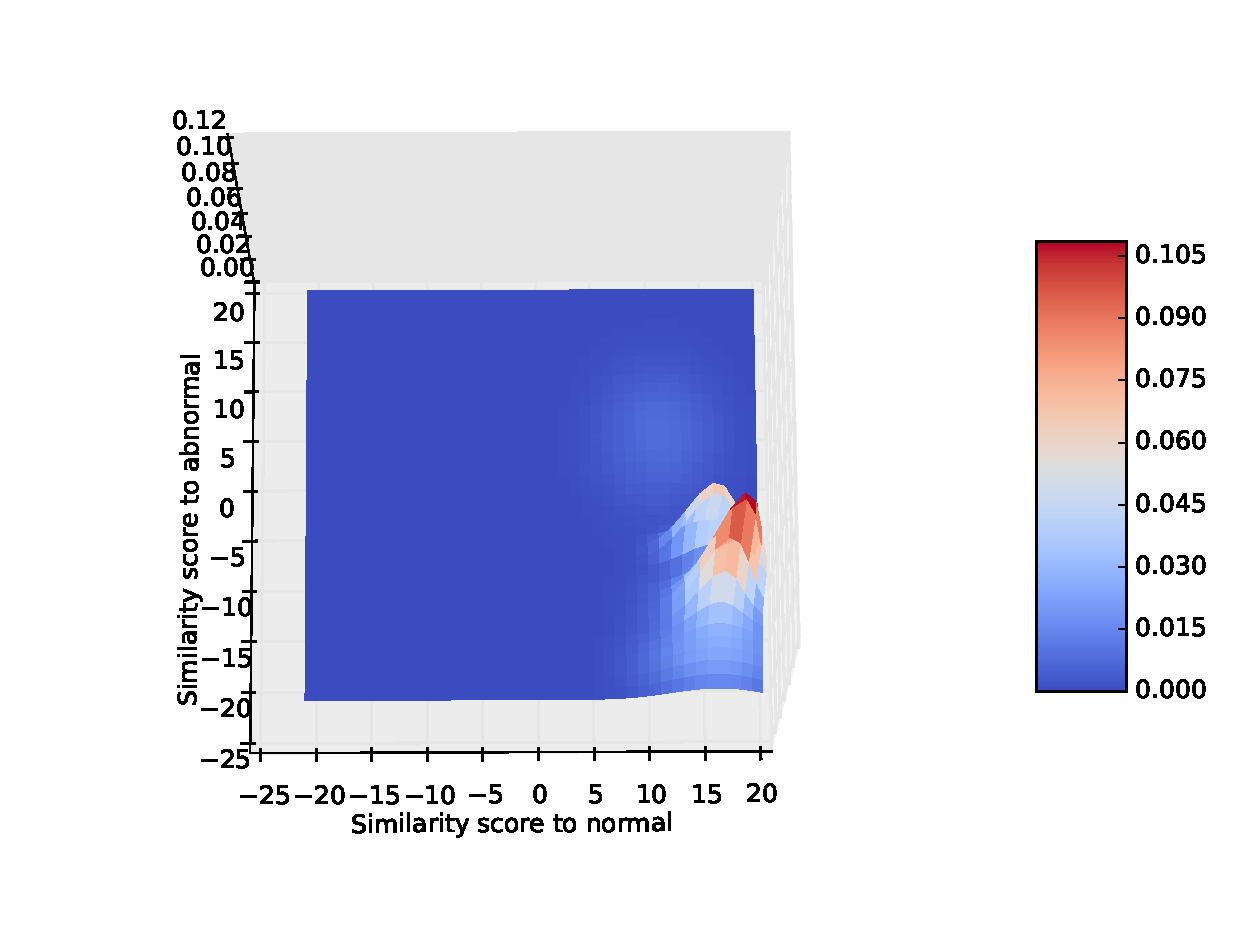
\includegraphics[width=2.0in,angle=0]{./sections/guess.eps}}
\end{center}
\caption{Density based intrusion detection result for unknown anomalies.  Red:Known and seen abnormal connections, Green:Known and seen normal connections, Blue:Intrusion \textit{snmpguess} which is a unknown anomaly similar to normal connections.} % I may show rest of data in appendix
\label{fig:refSingleRobot1}
\end{figure}

The performance of density approach is not as good as previous one, and we can see that it is not able to detect \textit{sendmail} class which is too few to form enough density. 
\begin{table}[h]
\begin{center}
\scalebox{0.7}{
\begin{tabular}{| l | l | l | l | l | l | p{5cm} |}
\hline
Type of Anomaly & The number of anomalies & TP & TN & FP & FN & Detection rate ($\%$ correct) \\
\hline
snmpguess & 1293 (331) & 975 & 1182 (254) & 111 (77) & 63 & 93.9 (76.7) \\ 
\hline
snmpgetattack & 1140 (178) & 973 & 1048 (126) & 92 (52) & 65 & 91.19 (71.5) \\
\hline
mailbomb & 1255 (293) & 882 & 1133 (223) & 122 (70) & 156 & 90.2 (76.1) \\
\hline
sendmail & 976 (14) & 1019 & 907 (0) & 69 (14) & 19 & 92.9 (0) \\
\hline
\end{tabular}
}
\end{center}
\caption{Detection result of unknown anomalies that is similar to known normal connections. The number in parentheses refers specific anomaly type.}
\label{fig:refSingleRobot1}
\end{table}

%4 out of 17 are close to known normal connections. 
%We can not detect them with exactly same way what it have done to known anomalies since abnormal and normal connections are mixed together. 
%However we can differenciate with density approach after the spectral clustering. 
%Here is the result, and their performance is good. 
%\begin{table}[h]
%\begin{center}
%\begin{tabular}{| l | l | l | p{5cm} |}
%\hline
%Type of Anomaly & Predicted normal & Predicted anormalies & $\%$ correct\\
%\hline
%True normal &  &  & \\
%\hline
%True anormalies (close to A)&  &  & \\
%\hline
%True anormalies (close to N) &  &  & \\
%\hline
%\end{tabular}
%\end{center}
%\caption{Abnomal classes in NSL-KDD99}
%\label{fig:refSingleRobot1}
%\end{table}
%\begin{table}[h]
%\begin{center}
%\begin{tabular}{| l | l | p{5cm} |}
%\hline
%Type of Anomaly & Count & $ \%$ correct\\
%\hline
%guess passwd & 100 & 80 \\
%\hline
%ftp write & 3 & 66.66 \\
%\hline
%nmap & 73 & 85.71 \\
%\hline
%back & 100 & 98.03  \\
%\hline
%multihop & 18 & 100  \\
%\hline
%rootkit & 13 & 84.61  \\
%\hline
%pod & 41 & 100  \\
%\hline
%perl & 2 & 0  \\
%\hline
%ipsweep & 117 & 97.4  \\
%\hline
%teardrop & 12 & 100  \\
%\hline
%satan & 100 & 87.96  \\
%\hline
%loadmodule & 2 & 0  \\
%\hline
%buffer overflow & 20 & 90  \\
%\hline
%phf & 2 & 50  \\
%\hline
%warezmaster & 100 & 84  \\
%\hline
%imap & 1 & 100  \\
%\hline
%warezclient & 6 & 0  \\
%\hline
%land & 7 & 100  \\
%\hline
%neptune & 100 & 100  \\
%\hline
%smurf & 100 & 100  \\
%\hline
%processtable & 100 & 100  \\
%\hline
%named & 17 & 88  \\
%\hline
%udpstorm & 2 & 100  \\
%\hline
%snmpguess & 100 & 72  \\
%\hline
%sqlattack & 2 & 100  \\
%\hline
%ps & 15 & 100  \\
%\hline
%httptunnel & 100 & 81  \\
%\hline
%sendmail & 14 & 0  \\
%\hline
%snmpgetattack & 100 & 97  \\
%\hline
%apache2 & 100 & 100  \\
%\hline
%saint & 100 & 98  \\
%\hline
%mailbomb & 100 & 72  \\
%\hline
%mscan & 100 & 100  \\
%\hline
%xterm & 13 & 100  \\
%\hline
%worm & 2 & 0  \\
%\hline
%xclock & 9 & 88.88  \\
%\hline
%xsnoop & 4 & 0  \\
%\end{tabular}
%\end{center}
%\caption{Abnomal classes in NSL-KDD99}
%\label{fig:refSingleRobot1}
%\end{table}
